\documentclass[aspectratio=169]{beamer}
\usetheme{Madrid}
\usecolortheme{seagull}
\usepackage{graphicx}
\usepackage{hyperref}
\usepackage{booktabs}
\usepackage{tikz}
\usetikzlibrary{positioning}

\title{A Conversational AI Agent for FIB}
\subtitle{Hierarchical Design and LLM-as-Judge Evaluation}
\author[Ákos Schneider, Ignasi Cervero]{Ákos Schneider \and Ignasi Cervero}
\institute[]{Facultat d'Informàtica de Barcelona\\Universitat Politècnica de Catalunya}
\date{Human Language Engineering}

\setbeamertemplate{navigation symbols}{}
\setbeameroption{hide notes}

% Custom colors
\definecolor{upcblue}{RGB}{0, 64, 128}
\setbeamercolor{title}{fg=upcblue}
\setbeamercolor{frametitle}{fg=upcblue}

\begin{document}

% =============================================================================
% SLIDE 1: Title
% =============================================================================
\begin{frame}
  \titlepage
  \note{Welcome everyone. Today we present our conversational AI agent for FIB that allows students to query academic information using natural language.}
\end{frame}

% =============================================================================
% SLIDE 2: The Problem
% =============================================================================
\begin{frame}{The Problem: Fragmented Academic Information}
  \begin{columns}[T,onlytextwidth]
    \begin{column}{0.52\textwidth}
      \textbf{Students face multiple challenges:}
      \vspace{0.5em}
      \begin{itemize}
        \item Data scattered across Racó, FIB API, and website
        \item Simple queries require many clicks
        \item No system understands implicit context
        \item Real-time info critical during exams
      \end{itemize}
      \vspace{1em}
      \textbf{Example:} ``When is my next exam?''
      \begin{itemize}
        \item[$\rightarrow$] Check enrolled courses
        \item[$\rightarrow$] Navigate to exam section
        \item[$\rightarrow$] Filter by your courses
        \item[$\rightarrow$] Compare dates manually
      \end{itemize}
    \end{column}
    \begin{column}{0.45\textwidth}
      \centering
      \includegraphics[width=\linewidth,height=0.75\textheight,keepaspectratio]{assets/s02_problem.png}
    \end{column}
  \end{columns}
  \note{Students navigate multiple fragmented systems. A simple question like 'When is my next exam?' requires knowing your courses, finding exams for each, and comparing dates - tedious!}
\end{frame}

% =============================================================================
% SLIDE 3: Our Solution
% =============================================================================
\begin{frame}{Our Solution: Natural Language Interface}
  \begin{columns}[T,onlytextwidth]
    \begin{column}{0.52\textwidth}
      \textbf{A conversational AI agent that:}
      \vspace{0.5em}
      \begin{itemize}
        \item Understands natural language queries
        \item Integrates with the official FIB API
        \item Handles implicit context automatically
        \item Supports both public and private data
      \end{itemize}
      \vspace{1em}
      \textbf{Now you can just ask:}
      \begin{itemize}
        \item ``When is my next exam?''
        \item ``What do I have tomorrow?''
        \item ``How many credits is IA?''
        \item ``Who teaches EDA?''
      \end{itemize}
    \end{column}
    \begin{column}{0.45\textwidth}
      \centering
      \includegraphics[width=\linewidth,height=0.75\textheight,keepaspectratio]{assets/s03_solution.png}
    \end{column}
  \end{columns}
  \note{Our solution is a conversational agent that understands context. 'What do I have tomorrow?' just works - the agent figures out your courses and schedule automatically.}
\end{frame}

% =============================================================================
% SLIDE 4: Architecture Overview
% =============================================================================
\begin{frame}{Architecture: Hierarchical Agent Design}
  \begin{columns}[T,onlytextwidth]
    \begin{column}{0.48\textwidth}
      \textbf{Two-level hierarchy:}
      \vspace{0.5em}
      \begin{itemize}
        \item \textbf{Root Agent}
        \begin{itemize}
          \item User context \& authentication
          \item Private tools (OAuth)
          \item Internet search fallback
          \item Task delegation
        \end{itemize}
        \vspace{0.5em}
        \item \textbf{Public Subagent}
        \begin{itemize}
          \item Specialized for FIB API
          \item Focused system prompt
          \item Public data queries
        \end{itemize}
      \end{itemize}
      \vspace{0.5em}
      \textbf{Benefits:} Focused prompts, security boundary, modularity
    \end{column}
    \begin{column}{0.50\textwidth}
      \centering
      \includegraphics[width=\linewidth,height=0.78\textheight,keepaspectratio]{assets/s04_architecture.png}
    \end{column}
  \end{columns}
  \note{We use a hierarchical design. The root agent handles user context and private tools, delegating public queries to a specialized subagent. This separation provides focused prompts and security boundaries.}
\end{frame}

% =============================================================================
% SLIDE 4b: Architecture (Full Screen)
% =============================================================================
\begin{frame}[plain]
  \centering
  \includegraphics[width=0.92\textwidth,height=0.92\textheight,keepaspectratio]{assets/architecture.png}
\end{frame}

% =============================================================================
% SLIDE 5: The Tool Ecosystem
% =============================================================================
\begin{frame}{The Tool Ecosystem}
  \begin{columns}[T,onlytextwidth]
    \begin{column}{0.48\textwidth}
      \textbf{Public Tools} (FIB API)
      \vspace{0.3em}
      \begin{itemize}
        \item \texttt{search\_courses} -- Find courses by name/code
        \item \texttt{get\_course\_details} -- Full course info
        \item \texttt{search\_exams} -- Exam schedules
        \item \texttt{search\_professors} -- Faculty search
        \item \texttt{get\_fib\_news} -- Announcements
        \item \texttt{list\_classrooms} -- Room info
      \end{itemize}
    \end{column}
    \begin{column}{0.48\textwidth}
      \textbf{Private Tools} (OAuth required)
      \vspace{0.3em}
      \begin{itemize}
        \item \texttt{get\_my\_profile} -- User info
        \item \texttt{get\_my\_courses} -- Enrolled courses
        \item \texttt{get\_my\_schedule} -- Personal timetable
        \item \texttt{get\_my\_notices} -- Course notices
      \end{itemize}
      \vspace{1em}
      \textbf{External}
      \begin{itemize}
        \item \texttt{internet\_search} -- Tavily API
      \end{itemize}
    \end{column}
  \end{columns}
  \vspace{0.5em}
  \centering
  \small All tools are typed Python functions with Pydantic validation
  \note{We wrap each API endpoint as a typed Python function. Public tools handle general queries, private tools require OAuth for user-specific data, and we have internet search as fallback.}
\end{frame}

% =============================================================================
% SLIDE 6: How It Works - ReAct Loop
% =============================================================================
\begin{frame}{How It Works: The ReAct Loop}
  \begin{columns}[T,onlytextwidth]
    \begin{column}{0.48\textwidth}
      \textbf{Reasoning + Acting paradigm:}
      \vspace{0.5em}
      \begin{enumerate}
        \item \textbf{Thought} -- Reason about the query
        \item \textbf{Action} -- Call appropriate tool
        \item \textbf{Observation} -- Process result
        \item \textbf{Repeat} until answer ready
      \end{enumerate}
      \vspace{1em}
      \textbf{Example thought process:}
      \begin{itemize}
        \item[$\rightarrow$] ``User wants exam info''
        \item[$\rightarrow$] ``Need their enrolled courses first''
        \item[$\rightarrow$] Call \texttt{get\_my\_courses()}
        \item[$\rightarrow$] ``Got [BD, EDA, IA], now search exams''
      \end{itemize}
    \end{column}
    \begin{column}{0.50\textwidth}
      \centering
      \includegraphics[width=\linewidth,height=0.78\textheight,keepaspectratio]{assets/s06_agentflow.png}
    \end{column}
  \end{columns}
  \note{The agent follows the ReAct paradigm - interleaving reasoning with actions. It thinks about what's needed, calls tools, observes results, and iterates until it can answer.}
\end{frame}

% =============================================================================
% SLIDE 6b: Agent Flow (Full Screen)
% =============================================================================
\begin{frame}[plain]
  \centering
  \includegraphics[width=0.92\textwidth,height=0.92\textheight,keepaspectratio]{assets/agent-flow.png}
\end{frame}

% =============================================================================
% SLIDE 7: Live Example Flow
% =============================================================================
\begin{frame}{Example: ``When is my next exam?''}
  \centering
  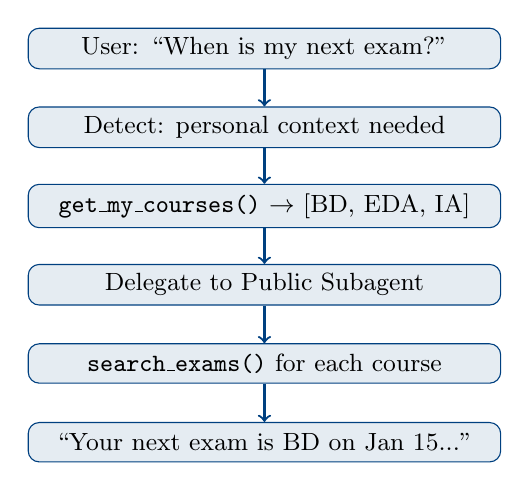
\begin{tikzpicture}[
    box/.style={rectangle, draw=upcblue, fill=upcblue!10, rounded corners, minimum width=6cm, minimum height=0.5cm, align=center, font=\small},
    arrow/.style={->, thick, upcblue}
  ]
    \node[box] at (0, 0)    (user)     {User: ``When is my next exam?''};
    \node[box] at (0, -1)   (detect)   {Detect: personal context needed};
    \node[box] at (0, -2)   (courses)  {\texttt{get\_my\_courses()} $\rightarrow$ [BD, EDA, IA]};
    \node[box] at (0, -3)   (delegate) {Delegate to Public Subagent};
    \node[box] at (0, -4)   (exams)    {\texttt{search\_exams()} for each course};
    \node[box] at (0, -5)   (response) {``Your next exam is BD on Jan 15...''};
    
    \draw[arrow] (user) -- (detect);
    \draw[arrow] (detect) -- (courses);
    \draw[arrow] (courses) -- (delegate);
    \draw[arrow] (delegate) -- (exams);
    \draw[arrow] (exams) -- (response);
  \end{tikzpicture}
  \note{Let's trace through a real example. The user asks about their next exam. The agent detects personal context is needed, gets enrolled courses, delegates exam search to the subagent, and returns the answer.}
\end{frame}

% =============================================================================
% SLIDE 8: Prompt Engineering Highlights
% =============================================================================
\begin{frame}{Prompt Engineering Highlights}
  \begin{columns}[T,onlytextwidth]
    \begin{column}{0.52\textwidth}
      \textbf{Key techniques in system prompts:}
      \vspace{0.5em}
      \begin{itemize}
        \item \textbf{Context detection}
        \begin{itemize}
          \item ``my exam'' $\rightarrow$ check enrolled courses first
          \item ``tomorrow'' $\rightarrow$ resolve to weekday
        \end{itemize}
        \vspace{0.3em}
        \item \textbf{Date reasoning}
        \begin{itemize}
          \item Explicit weekday mappings (Monday=1)
          \item Current date in context
        \end{itemize}
        \vspace{0.3em}
        \item \textbf{Disambiguation strategy}
        \begin{itemize}
          \item ``Machine Learning'' $\rightarrow$ multiple matches
          \item Present top options, ask for clarification
        \end{itemize}
        \vspace{0.3em}
        \item \textbf{Quality checklist} before responding
      \end{itemize}
    \end{column}
    \begin{column}{0.45\textwidth}
      \centering
      \includegraphics[width=\linewidth,height=0.75\textheight,keepaspectratio]{assets/s08_prompts.png}
    \end{column}
  \end{columns}
  \note{Prompt engineering is crucial. We handle implicit context, provide date mappings so the agent doesn't need internet search, and define strategies for ambiguous queries.}
\end{frame}

% =============================================================================
% SLIDE 9: Evaluation Framework
% =============================================================================
\begin{frame}{Evaluation: LLM-as-Judge Framework}
  \begin{columns}[T,onlytextwidth]
    \begin{column}{0.48\textwidth}
      \textbf{Why LLM-as-Judge?}
      \begin{itemize}
        \item Traditional metrics (BLEU, ROUGE) correlate poorly with quality
        \item LLM judges understand semantic meaning
        \item Custom rubrics for each metric
      \end{itemize}
      \vspace{0.5em}
      \textbf{Our setup:}
      \begin{itemize}
        \item 45 curated test questions
        \item 10 categories of queries
        \item 7 evaluation metrics
        \item Gemini 2.5 Flash Lite as judge
      \end{itemize}
    \end{column}
    \begin{column}{0.50\textwidth}
      \centering
      \includegraphics[width=\linewidth,height=0.78\textheight,keepaspectratio]{assets/s09_evaluation.png}
    \end{column}
  \end{columns}
  \note{We use LLM-as-judge because traditional metrics don't capture response quality well. We have 45 questions, 7 metrics, and detailed rubrics for consistent evaluation.}
\end{frame}

% =============================================================================
% SLIDE 9b: Evaluation Pipeline (Full Screen)
% =============================================================================
\begin{frame}[plain]
  \centering
  \includegraphics[width=0.92\textwidth,height=0.92\textheight,keepaspectratio]{assets/evaluation-pipeline.png}
\end{frame}

% =============================================================================
% SLIDE 10: Question Categories & Metrics
% =============================================================================
\begin{frame}{Evaluation Dataset \& Metrics}
  \begin{columns}[T,onlytextwidth]
    \begin{column}{0.48\textwidth}
      \textbf{Question Categories}
      \vspace{0.3em}
      \begin{table}
        \footnotesize
        \begin{tabular}{lr}
          \toprule
          Category & Count \\
          \midrule
          courses & 13 \\
          exams & 5 \\
          professors & 4 \\
          personal (OAuth) & 4 \\
          multi\_tool & 5 \\
          ambiguous & 4 \\
          news, academic, etc. & 10 \\
          \bottomrule
        \end{tabular}
      \end{table}
      \vspace{0.3em}
      \textbf{Complexity:} Simple, Multi-step, Contextual, Ambiguous
    \end{column}
    \begin{column}{0.48\textwidth}
      \textbf{7 Evaluation Metrics}
      \vspace{0.3em}
      \begin{itemize}
        \item \textbf{Relevance} -- addresses the question?
        \item \textbf{Helpfulness} -- actionable \& useful?
        \item \textbf{Conciseness} -- appropriately brief?
        \item \textbf{Structure} -- well-organized?
        \item \textbf{Tone} -- professional?
        \item \textbf{Error Handling} -- graceful failures?
        \item \textbf{Tool Appropriateness} -- right tools?
      \end{itemize}
    \end{column}
  \end{columns}
  \note{Our dataset covers 10 categories and 4 complexity levels. Each response is scored on 7 metrics with detailed rubrics defining correct and incorrect behaviors.}
\end{frame}

% =============================================================================
% SLIDE 11: Results - The Numbers
% =============================================================================
\begin{frame}{Results: Meeting Our Targets}
  \begin{columns}[T,onlytextwidth]
    \begin{column}{0.48\textwidth}
      \textbf{Gemini 2.5 Flash Results}
      \vspace{0.3em}
      \begin{table}
        \footnotesize
        \begin{tabular}{lrrl}
          \toprule
          Metric & Score & Target & \\
          \midrule
          Relevance & 0.90 & $>$0.85 & \textcolor{green!60!black}{\checkmark} \\
          Helpfulness & 0.89 & $>$0.85 & \textcolor{green!60!black}{\checkmark} \\
          Conciseness & 0.85 & $>$0.80 & \textcolor{green!60!black}{\checkmark} \\
          Structure & 0.77 & $>$0.75 & \textcolor{green!60!black}{\checkmark} \\
          Tone & 0.85 & $>$0.80 & \textcolor{green!60!black}{\checkmark} \\
          Error Handling & 0.51 & $>$0.70 & \textcolor{red!70!black}{$\times$} \\
          Tool Approp. & 0.77 & $>$0.80 & \textcolor{orange!80!black}{$\sim$} \\
          \midrule
          \textbf{Average} & \textbf{0.79} & & \\
          \bottomrule
        \end{tabular}
      \end{table}
    \end{column}
    \begin{column}{0.48\textwidth}
      \textbf{Key Findings}
      \vspace{0.5em}
      \begin{itemize}
        \item Core metrics (relevance, helpfulness) exceed targets
        \item Flash vs Pro: nearly identical scores
        \item Flash recommended: faster, cheaper
      \end{itemize}
      \vspace{0.5em}
      \textbf{Top Categories (Relevance)}
      \begin{itemize}
        \item courses: 0.95
        \item academic: 0.95
        \item ambiguous: 0.93
        \item exams: 0.92
      \end{itemize}
    \end{column}
  \end{columns}
  \note{We meet targets on core metrics. Relevance and helpfulness - the most important for users - score 0.90 and 0.89. Error handling underperforms due to rubric issues we'll discuss.}
\end{frame}

% =============================================================================
% SLIDE 12: Lessons Learned
% =============================================================================
\begin{frame}{Lessons Learned}
  \begin{columns}[T,onlytextwidth]
    \begin{column}{0.52\textwidth}
      \textbf{Challenges \& Solutions}
      \vspace{0.5em}
      \begin{itemize}
        \item \textbf{Ambiguous queries}
        \begin{itemize}
          \item[$\rightarrow$] Present top matches first
          \item[$\rightarrow$] Then ask for clarification
        \end{itemize}
        \vspace{0.3em}
        \item \textbf{Date-relative queries}
        \begin{itemize}
          \item[$\rightarrow$] Explicit date in context
          \item[$\rightarrow$] Weekday mappings in prompt
        \end{itemize}
        \vspace{0.3em}
        \item \textbf{Error handling scored low}
        \begin{itemize}
          \item[$\rightarrow$] Rubric was overly strict
          \item[$\rightarrow$] Agent too verbose on errors
        \end{itemize}
        \vspace{0.3em}
        \item \textbf{Tool tracking across subagents}
        \begin{itemize}
          \item[$\rightarrow$] Evaluation sees only ``task'' call
          \item[$\rightarrow$] Need trajectory flattening
        \end{itemize}
      \end{itemize}
    \end{column}
    \begin{column}{0.45\textwidth}
      \centering
      \includegraphics[width=\linewidth,height=0.75\textheight,keepaspectratio]{assets/s12_lessons.png}
    \end{column}
  \end{columns}
  \note{Key lessons: handle ambiguity by offering options first, provide date context explicitly, and be aware that hierarchical architectures complicate tool tracking in evaluation.}
\end{frame}

% =============================================================================
% SLIDE 13: Contributions & Future Work
% =============================================================================
\begin{frame}{Contributions \& Future Work}
  \begin{columns}[T,onlytextwidth]
    \begin{column}{0.52\textwidth}
      \small
      \textbf{Contributions}
      \vspace{0.2em}
      \begin{itemize}
        \setlength{\itemsep}{0.1em}
        \item Open-source FIB Agent with hierarchical architecture
        \item 45-question evaluation dataset (10 categories)
        \item Reusable LLM-as-judge framework
        \item MCP server for AI interoperability
        \item Documented prompt engineering patterns
      \end{itemize}
      \vspace{0.3em}
      \textbf{Future Directions}
      \vspace{0.2em}
      \begin{itemize}
        \setlength{\itemsep}{0.1em}
        \item RAG with syllabi \& lecture notes
        \item Conversation memory (multi-turn)
        \item User interface (Telegram bot, web chat)
        \item Multi-university adaptation
      \end{itemize}
    \end{column}
    \begin{column}{0.45\textwidth}
      \centering
      \includegraphics[width=\linewidth,height=0.75\textheight,keepaspectratio]{assets/s13_future.png}
    \end{column}
  \end{columns}
  \note{Our contributions include the agent, dataset, evaluation framework, and MCP server. Future work includes RAG for richer answers, conversation memory, and user-facing interfaces.}
\end{frame}

% =============================================================================
% SLIDE 14: Thank You / Q&A
% =============================================================================
\begin{frame}{Thank You}
  \begin{columns}[T,onlytextwidth]
    \begin{column}{0.55\textwidth}
      \vspace{1em}
      \textbf{Key Takeaway}
      \vspace{0.5em}
      \begin{quote}
        ``Modern LLM agents can effectively serve as natural language interfaces to structured APIs when properly configured with domain-specific tools and engineered prompts.''
      \end{quote}
      \vspace{1em}
      \textbf{Links}
      \begin{itemize}
        \item FIB API: \url{https://api.fib.upc.edu/v2/}
        \item LangGraph: \url{https://langchain-ai.github.io/langgraph/}
        \item deepagents: \url{https://github.com/langchain-ai/deepagents}
      \end{itemize}
      \vspace{1em}
      \centering
      \Large Questions?
    \end{column}
    \begin{column}{0.42\textwidth}
      \centering
      \includegraphics[width=\linewidth,height=0.75\textheight,keepaspectratio]{assets/s14_thankyou.png}
    \end{column}
  \end{columns}
  \note{Thank you for your attention. The key message is that LLM agents with proper tooling and prompts can serve as effective natural language interfaces. Happy to take questions!}
\end{frame}

\end{document}
